\documentclass[a4paper]{article}

\usepackage[T1]{fontenc}
\usepackage[utf8]{inputenc}
\usepackage{lmodern}
\usepackage{graphicx}
\usepackage[english]{babel}
\usepackage{csquotes}

\usepackage[notes,backend=biber]{biblatex-chicago}
\bibliography{sample}

\begin{document}
\title{The Telepathy Guide Book for Dummies}
\author{Tongda Xu}
\maketitle

\begin{abstract}

Telepathy, as coined word used to be popular in Gothic imagination and psychoanalysis, is reused by recent scholars and converted into ideas such as \textit{implicit interaction} or \textit{silent speech}. This paper rediscover the concept of telepathy , the modern implement of telepathy and discuss two possible new implement of telepathy in modern Brain-computer Interface (BCI) context.

This paper describe design and implement of two telepathy applications based on two popular BCI paradigms respectively: ERP(Event-Related Potentials) and ERD/ERS (Event-Related De/Synchronizations). The first one typically involves the immediate potential change after the stimulation of certain frequency of flash light, which could be decoded into binary signal for text-based communication. The second one could be feeded into machine learning model to regress measure a mid-term emotional state for emotion sharing.  
\end{abstract}

\section{Introduction}

The word telepathy, coined in 1882 by poet Frederic Myers: "we venture to introduce the words \textit{Telaethesia} and \textit{Telepathy} to cover all cases of impression received at a distance" \autocite{luckhurst2002invention}. It was initially defined as \textit {forms of occult relation or communication between people at distance}. \autocite{luckhurst2002invention} It was proposed with the wave of modernism and deeply  strongly connected with Gothic imagination, mother's hyper-sensitivity and psycho-analysis \autocite{freud1955dreams}.

\subsection{the Concept of Telepathy}

Unlike other coined concept such as mattiods or vortex atoms, telepathy broke into culture and bloomed quickly and is still popular in present days \autocite{luckhurst2002invention}, as a fancy metaphor for research scientists. But back to 1900s, the relationship between telepathy and science was quite different. Contemporary scientists focus on implementation of telepathy, regarding it as a far dream where people could interact naturally at distance fluently with aid of technology. 

Far before the existence of science, the record of telepathy had appeared in religious background, either as a privilege of God, such as \textit{Then the LORD saw that the wickedness of man was great on the earth, and that every intent of the thoughts of his heart was only evil continually} (Genesis 6:5) or as a sign of strong connection and familiarity between people, such as \textit{Behold, I know your thoughts, and the plans by which you would wrong me}(Job 21:27).

By the time science itself was born in late 1800s, all those phenomena were explained religiously. Since the science clubs were constituted as \textit{pure free, untrammelled by religious dogmas} \autocite{feist2017religion}, the naturalism (proper observation and experimental condition) was the dominant trend. On the other hand, there was another stream of scientists went against the naturalism, focusing on the study and application of super natural phenomena, they were called spiritualism. The naturalism and spiritualism hated each other, both hated and hated by the Church. It wasn't decades of fighting until 1879 the two groups settled down and collaborated on psychical research, that is also a period when psychological became a part of science subject. It was easy to explain why the initial scientific research on telepathy was all about explaining the telepathy experienced by people, claiming or counter claiming the existence of telepathy in the world\autocite{luckhurst2002invention} and analyzing the experience of telepathy psychologically. Since it was a balanced result among two groups of research scientists and church. 

Under this background, the first case of telepathy was proposed in science community on a journal of psychical research by William Barrett\autocite{luckhurst2002invention}. In a paper named \textit{On some phenomena associated with abnormal conditions of mind}, he described an abnormal experience that a peasant girl never go beyond the village could describe her memory in mind on Regent Street. \autocite{barrett1882some} Barrett explained as "the nervous action associated with thought can be excited by a corresponding action...across space and without the intervention of recognized organs of sensation."\autocite{luckhurst2002invention}.

Although the anecdote itself sounds like television, Barrett had given a very provisional explanation that coincides with modern brain-computer interface, which wasn't proposed until early 1970s, as "measuring brain activity ... BCI bypasses the brain’s normal output channels of peripheral nerves and muscles."\autocite{zander2014towards} The point here is central nerve in some way bypass peripheral nerves, either send or receive information. 

The collection of those personal experience report continued through 1880s, until first report on telepathy experiment in laboratory appear in 1883. The Creecy sisters with two subjects went through over 1000 supervised trails \autocite{luckhurst2002invention} of transmit words, numbers and images from various distance. Although denounced and condemned as "offensive incredulity" later, the results of experiments were positively acknowledged by the public.

\subsection{the Coining of Telepathy}

Despite the claiming and counter claiming the possibility of telepathy, another group of scientists were exploring the possibility of fancy remote communication method, coining the telepathy in a less fraud manner. An early example would be the Sympathetic resonance in John Tyndall's \textit{Sound} \autocite{tyndall1897sound}.

As a fancy demo in 1800s, the sympathetic resonance is no more than two fork resonating one another, just the behaviour is magnified in a interesting manner.Two small mirror is installed on each fork respectively. When one fork is hit, the resonance of two forks would be zoomed as the change of lighting pattern on the screen. 

Although this was a simple physical experiment in eye of contemporary people, it was quite a shocking demo in 18 century. And it was quite well known in the telepathy community as an evidence. Although the analogy is very confusing today, it was indeed the first popular wireless communication demo. The relationship between this demo and telepathy is simple. By that time people already known that mind movement are probably composed of electromagnetic wave. And since wave source would resonate with one another, the mind would resonate with each other, just as the forks. And people at that time were pretty satisfied with this ridiculous proof.

\begin{figure}
	\centering
	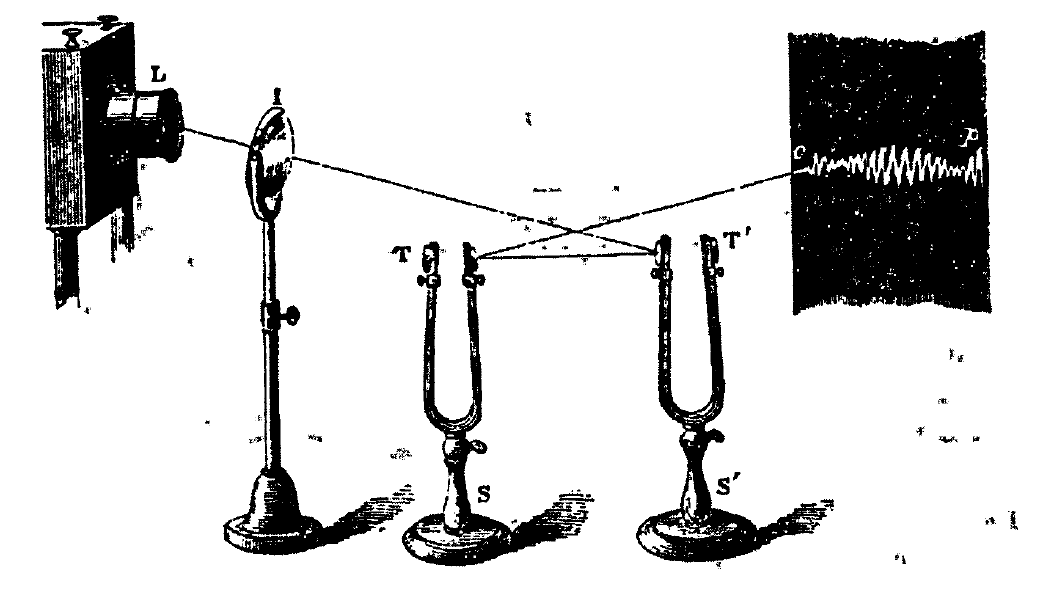
\includegraphics[width= \linewidth]{Sound1}
	\caption{Sympathetic resonance in John Tyndall's Sound}
	\label{fig:Sound1}
\end{figure}

\begin{figure}
	\centering
	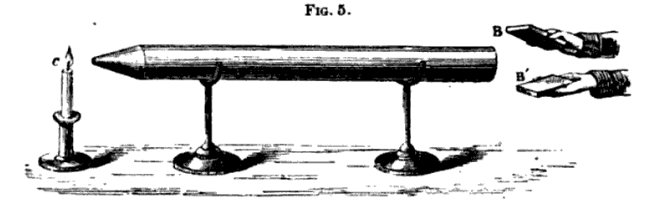
\includegraphics[width= \linewidth]{Sound2}
	\caption{Another transmitting sound wave example in John Tyndall's Sound}
	\label{fig:Sound1}
\end{figure}

And regarded as the real foundation of wireless communication \autocite{bell1876improvement}, the Bell's telephone patent in 1876 did not considered to be a major contribution of telepathy research community by their colleagues. Probably because the device and method of interaction was quite disenchanted and straightforward to understand.

\begin{figure}
	\centering
	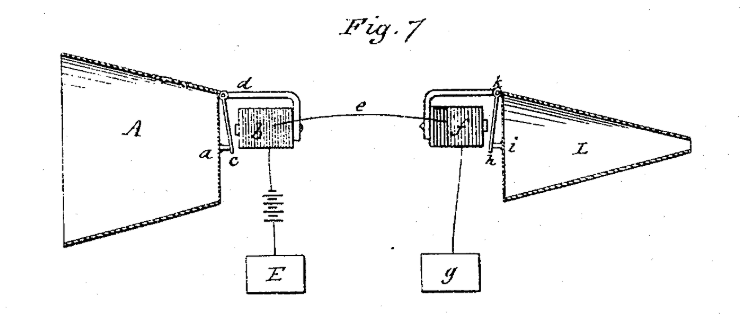
\includegraphics[width= \linewidth]{Bell}
	\caption{The Bell's patent on Improvement in telegraphy}
	\label{fig:Bell}
\end{figure}

Telephone for scientists was more practical, tangible and especially profitable. It really helped the communication between people and made inventors rich. Telepathy on the other hand, remained a black-box no matter how solid the scientist stated their founding was and how fancy was the story. Telepathy failed to evolve into a life changing industry since it could not be practiced successfully by everyone.

As Dobkin concluded, "I know that many men of light and discernment now regard telepathy as am established face, and in these days of wireless it would be rash to deny the possibility of it." \autocite{luckhurst2002invention}, many scholars suspect the possibility of real telepathy as superpower or mental phenomena. But they provisioned the realization of telepathy in era of wireless communication.

Although It is hard to say whether Dobkin admitted that his previous works was dubious. It would be clear that even the scientists working with telepathy at that time more or less suspected the soundness of it. After a long period of weird entanglement with science community, the concept of telepathy gradually faded out and dived into late Victorian Gothic fantasy, and served as a major topic in fictions for quite a long time.\autocite{luckhurst2002invention} It remains a deeply related concept with topic such as the woman sensitive and after-live.

\subsection{the Modern Implement of Telepathy}

It is not surprising that until recently telepathy has floated from the surface and noticed again by science community. A quite reasonable pathway of "tele-" technology should be telegraph, telephone, television, and finally telepathy. The difficulty of signal processing and band-width needed for communication increase all the way. And any telepathy demo before the mature of wireless communication is quite unsound. But it is not an overstatement that today, the technology is ready for telepathy.

The modern implement of Telepathy is generally more reasonable and practical than their eye-catching ancestors. The point shift from whether the super natural power of communication exist to make the users feel that it exist. In terms of initial point, the modern researcher disenchant the concept by technology and focus on the user's experience. The telegraph requires professional translation, telephone need manipulation to learn, but television (well I mean video call, not broadcasting) has evolved into a quite natural way of interaction. And telepathy, by no doubt, should be another level of user experience in terms of how natural and affordable the interaction is. 

If the communication is exchanging information or signal, the modern telepathy would first involve deliberate interruption of communication signal at different level. This interruption would produce different user experience. For example, the lip reading is the interruption of signal at speaking level (this could also be divided into 4 stages: Breathing, Phonation, Resonation and Articulation), brain computer interface based spelling is the interruption of signal at thought-muscle level. Then the interrupted signal is received, on the other hand, by artificial device, then being proceeded and used for future communication or interaction.

Another main difference is, thanks to NSF - National Science Foundation, modern telepathy start from practical use than unrealistic imagination. For example, one of the most important use of brain computer interface, so called motion imaginary, is widely applied for manipulation of wheel chair or artificial limb for those with physical inconvenience. And the start point of this technology, is building reimbursement equipment for the veterans who lost their legs in mining field of Vietnam \autocite{zander2014towards}. In terms of practical level, the telepathy has been disenchanted and stepped into professional service. Although not used by everyone, the mysterious cloak has been dismantled. 

\subsubsection{Interrupt Signal at Sound Level: Silent Speech Interface}

One of the major concern of voice interaction is keep the action of speech as not prominent as possible. For example, you are in a dinner with a couple of friends while you have to evoke the Siri, talking to Siri directly would bring awkwardness to both your friends and you.

\begin{figure}
	\centering
	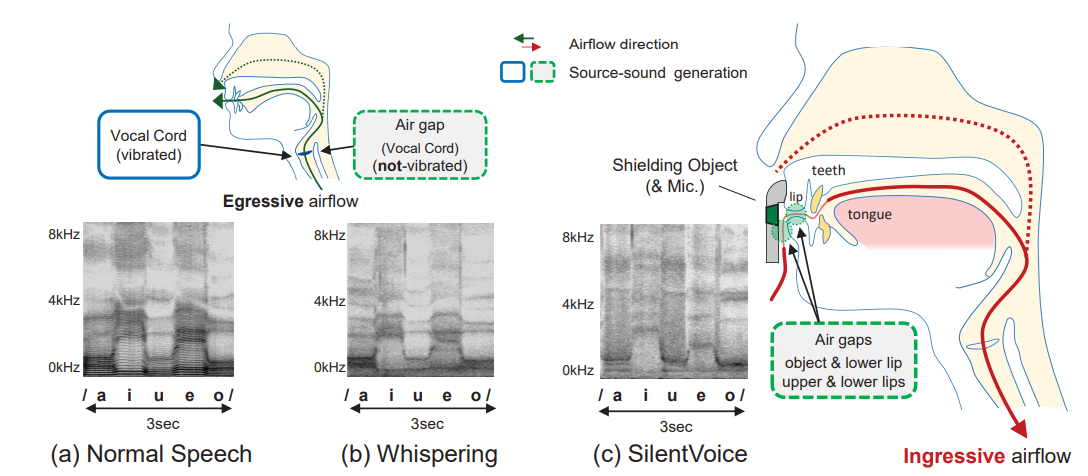
\includegraphics[width= \linewidth]{silentvoice}
	\caption{The silent-voice speaking technique by Dr. FUKUMOTO}
	\label{fig:P300}
\end{figure}

Group of scientist has contributed a lot to this silent speech area either by lip reading technique or by . One of the recent implement by Dr. FUKUMOTO allowing this special technique named silent-voice without demanding special microphones or communication devices \autocite{fukumoto2018silentvoice}.

Dr. FUKUMOTO introduced a speak method that change the exhale action of speaking into inhaling, in other words, ingressive speech. In this way, people could avoid the pop-noise and thus enhancing the signal/noise ratio of microphone. When performing silent-voice, the microphone device could be very near to mouth and provide more precision with very little noise making. And by commercial microphone device, the silent speech is 30 dB lower than normal speech, 20 dB lower than whispering while producing 5 dB louder signal, which promises a high communication efficiency avoiding noise making.  

\subsubsection{Interrupt Signal at Muscle Level: Electromyography Spelling/Lip Reading}

Another scenario where telepathy could be useful is: you want to talk to some one in the library but there are other people around you and making the noise could be really pricey, but you really have to talk to him because he forgets to wear his pants. Or you just spot someone about to hit a wall on street and performing silent-voice would be too hard and dramatic, mean while you would like some heavier device than daily microphone for the trade off: you could speak as usual without making sound, but you have to wear heavy device. Then electromyography (EMG) spelling would be a perfect fit.

EMG spelling generally involves the recognition of muscle potential when contracting and relaxing. When using EMG spelling, the process is more natural than silent speech. People just speak as usual but making no actual sound, the electrode would record the muscle movement and recognize the speech after Fourier Transformation proceeding, which is much easier than substituting all the exhale action to inhale.

An interesting implement of EMG spelling is by Dr. Bourland. The device is composed of 8 electrode EMG detector recording the muscle status around the mouth. Once the speech action is performed, the electrode would capture the signal and send to the server for analysis, which pretty fits into the paradigm of EMG spelling practice. The unique part is, the device also composes of Infrared sender and receiver. The send er is wore on the speaker's head and receiver's body. So the deciphered speaking content could be send to a desired location without bring noise to other person.  

\begin{figure}
	\centering
	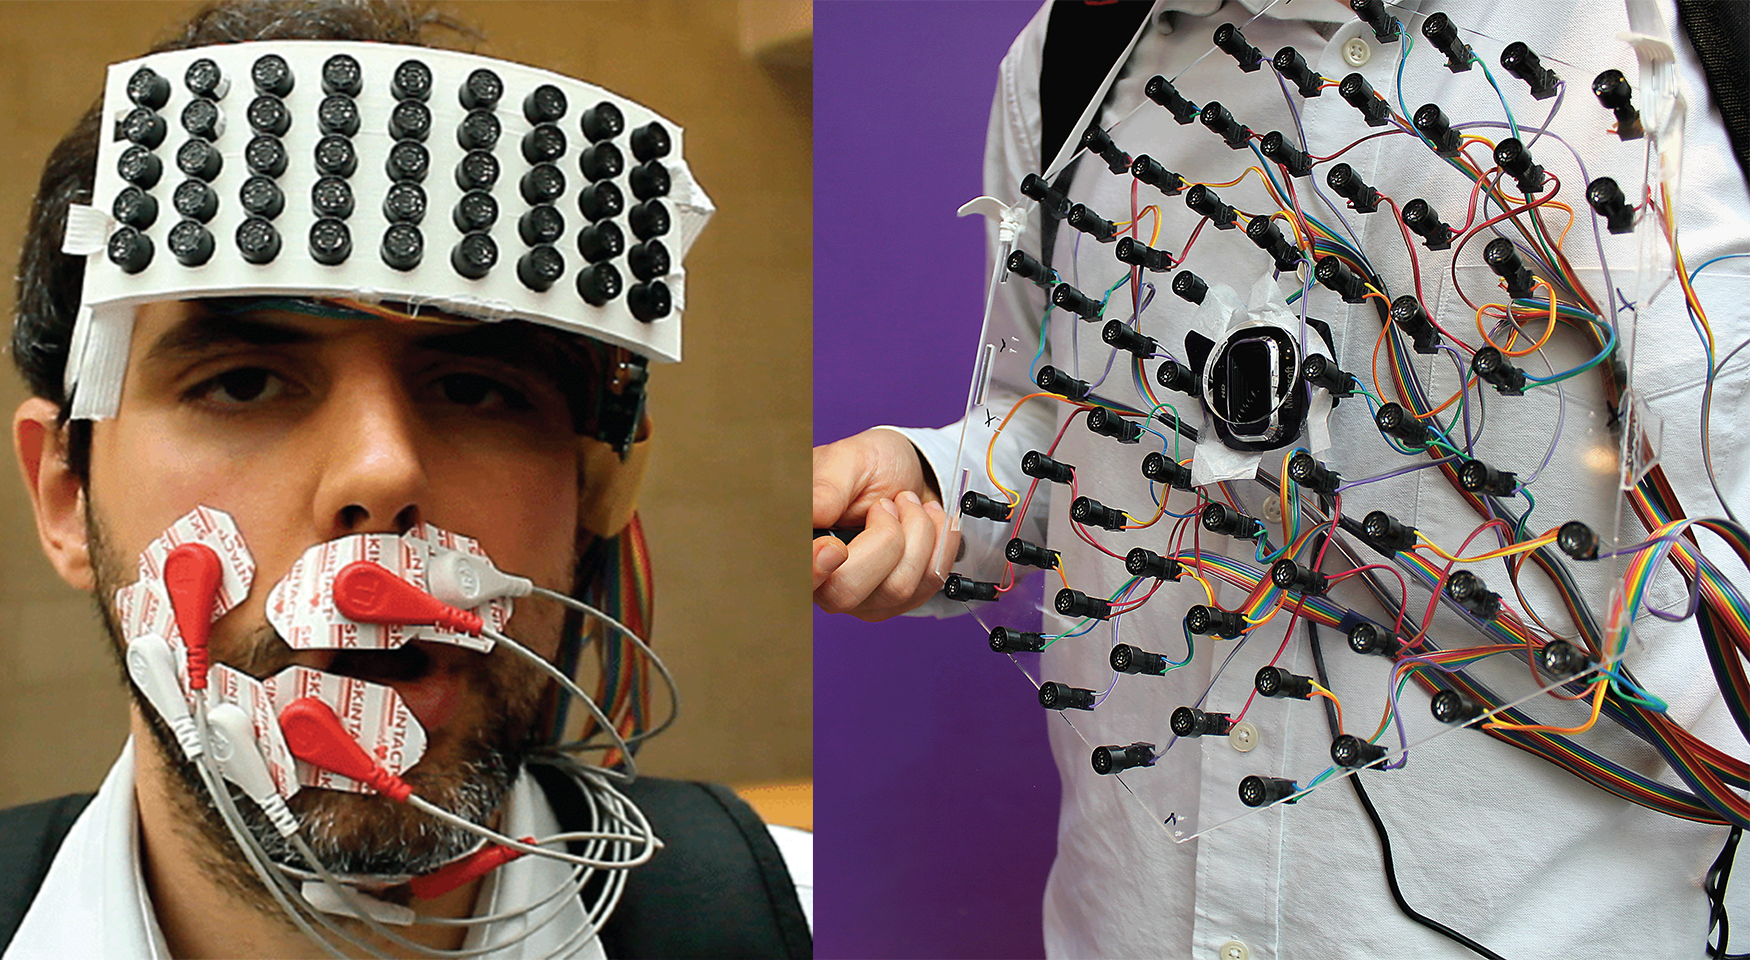
\includegraphics[width= \linewidth]{Proj_Tele}
	\caption{the implement of electromyography spelling by Dr. Bourland}
	\label{fig:Proj_Tele}
\end{figure}

Another approach to interrupt signal at muscle level is lip reading. As EMG spelling, the lip reading also requires subjects to speak as usual but not make actual sound. Then the image sequence would be captured by camera for further analysis in a standard modern computer vision fashion. A popular implement of processing lip image is CNN and LSTM. 

\begin{figure}
	\centering
	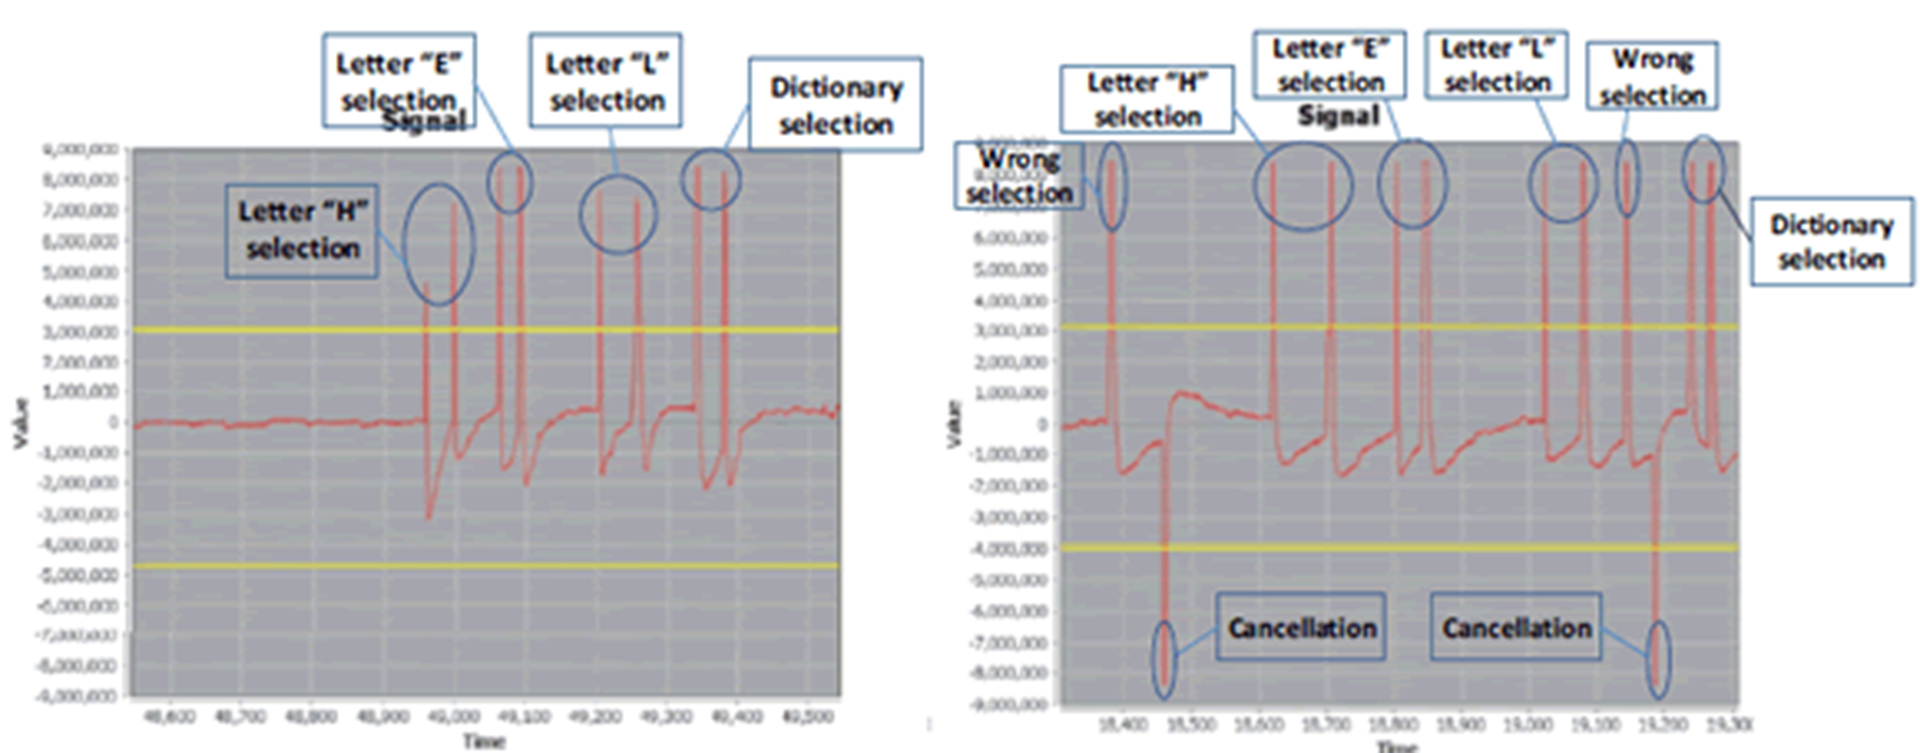
\includegraphics[width= \linewidth]{EMGSpell}
	\caption{the EMG signal when spelling \"hello\"}
	\label{fig:EMG}
\end{figure}

Stanford University offers a detailed implement \autocite{garg2016lip} and analysis of this technique using toy data set. The CNN network is used to extract the lip pose of a certain time, and LSTM is connected afterwards to handle a sequence of feature. The main limitation of this method is an external camera is needed and pose from a distance, which make the device loses the wearable trait. The major application is proposed as a manipulation interface through the front camera of smart phone, which is implement by Dr. Sun as a silent version of Siri.\autocite{sun2018lip} 

\begin{figure}
	\centering
	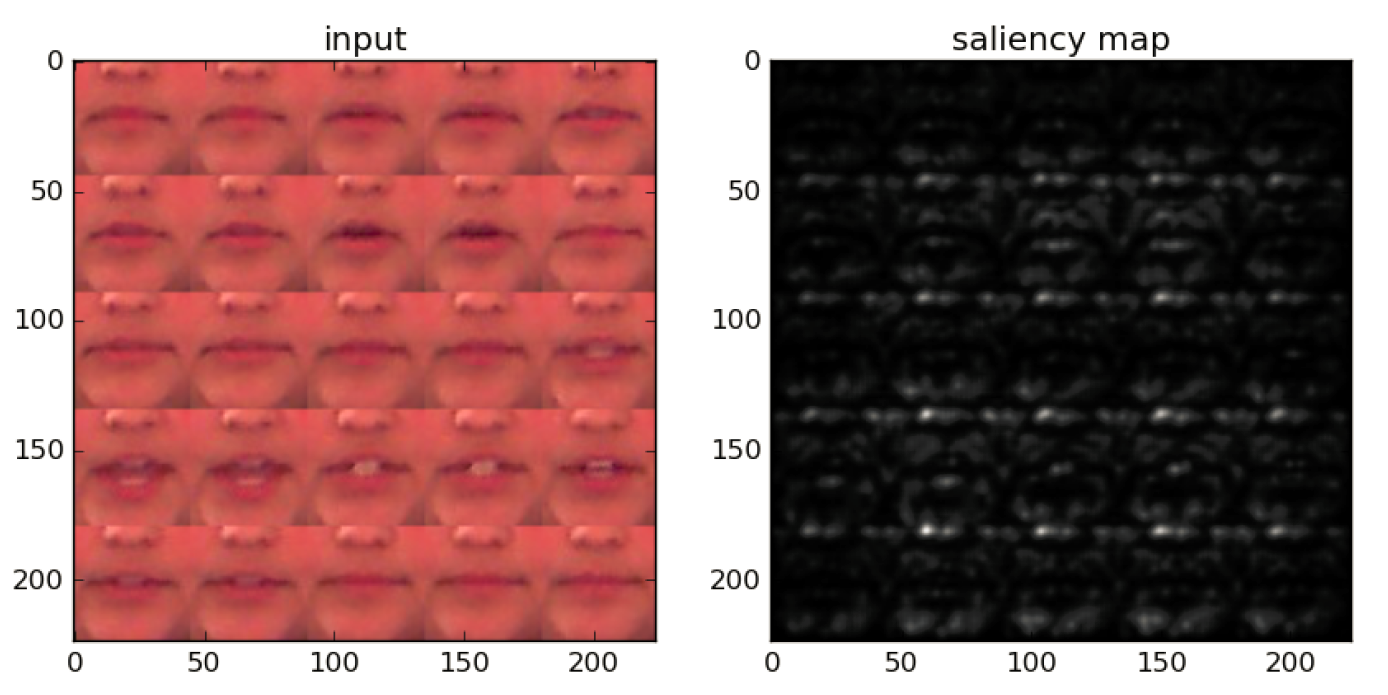
\includegraphics[width= \linewidth]{Lip}
	\caption{the feature extracted for different lip pose}
	\label{fig:lip}
\end{figure}

\subsubsection{Interrupt Signal at Central Nerve Level: Brain-computer Interface}

The trait of brain-computer interface is that it interrupt signal from central nerve system when transmitting to peripheral nerve system, which could be used to provide a much more implicit and natural interaction experience. Some time this interaction or input does not even have to be awarded of by the user. But the problem is that the device required is more complicated and the accuracy is not as good as the previous ones.

\begin{figure}
	\centering
	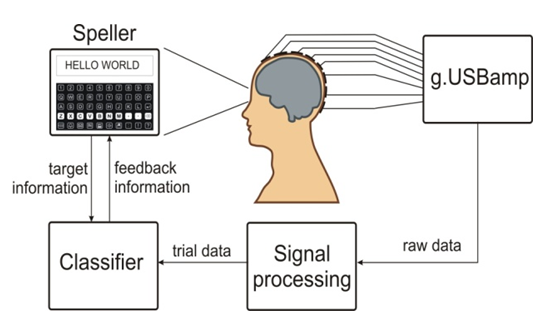
\includegraphics[width= 0.8 \linewidth]{P300Dia}
	\caption{a typical setup for P300 speller}
	\label{fig:300Spell}
\end{figure}


One good example of using brain computer interface is the P300 based spelling machine, which is commonly used as an alternative text input method for people having trouble speak or move their hand, A typical implement of P300 speller\autocite{krusienski2008toward} would requires a screen with a flashing alphabet matrix \autocite{sakai2012alphabet}. The people would implicitly choose the correct character they want to spell by choosing the row first than column (will be discussed in detail later).

\subsection{the Paradigm of modern Brain Computer Interface}

Although the idea of reading Electroencephalogram (EEG) could be traced back to 1929 \autocite{RN46}, the concept of brain-computer interface (BCI) was not proposed until early 1970s \autocite{RN48}. Initially, it was adopted to restore independence of people with neural pathways diseases. Since it could bypass the normal output of brain such as peripheral nerves and read signals directly \autocite{RN37}.

Nowadays, BCI has been freed from the original medical definition \autocite{RN37}. Instead of a "non-muscular communication and control channel for neuromuscular disabilities" \autocite{RN46}, BCI has expanded to serve general communication need of healthy people \autocite{RN37}. 

The advantage of using brain computer interface for telepathy is: ,

\begin{itemize}
\item First, it is hide deep enough since it interrupts the signal since central nerve system. This is coincident with the initial explanation of telepathy, that the central nerve system conducting action and interact with remote object without any muscle or other organ.
\item Second, it is involuntary and widely used for implicit interaction. This is parallel to the super natural trait of telepathy, such that the subject often reported haunted or found strange information in dream. The user could not control a large portion of brain-wave intentionally.
\end{itemize}

There are two major paradigm of adopting EEG signals: Event-Related Potentials(ERP) and Event-Related De/Synchronizations(ERD/ERS).\autocite{alarcao2017emotions}

\begin{figure}
	\centering
	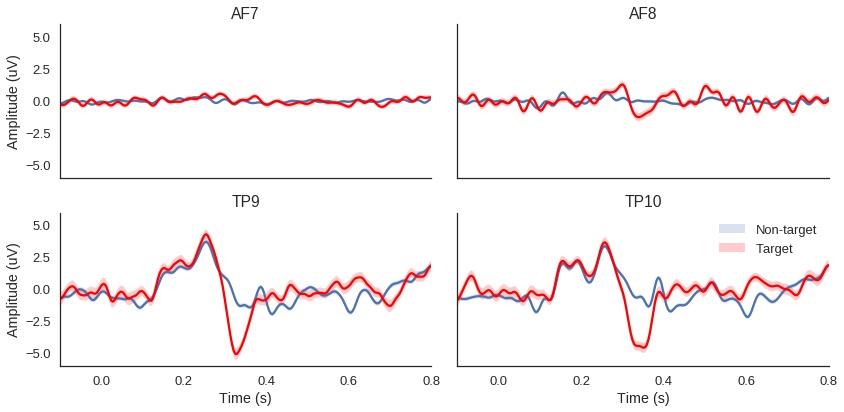
\includegraphics[width= 0.8\linewidth]{P300}
	\caption{An example of P300 signal from Dr. Alexandre Barachant}
	\label{fig:P300}
\end{figure}

Event-Related potential generally involves the change of electrical potential after sensory stimulation. Based on stimulation type, scholars cut them into subcategories such as Auditory Evoked Potentials (AEP), Visual Evoked Potentials (VEP) and Somatosensory Evoked Potentials (SsEP)\autocite{alarcao2017emotions}. VEP is typically implemented by giving a flash light or flash pattern on monitor to produce change of electrical potential on different electrodes location. VEP is elicited by a tone stimulus through earphones and SsEP by a direct electrical stimulation of nerve system. The ERP could provide high temporal resolution about the immediate influence of a brief stimuli. Among which P300, the positive deflection in voltage with a latency of roughly 250 to 500 ms is the most common signal used for VEP. 

ERD/ERS, on the other hand analysis the power change within certain frequency band of across electrodes. The increase of band power is defined as ERS while decrease as ERD. The ERD/ERS approach is commonly used for measuring the existing reaction to affection related communication, such as the emotion state of people or motion imaginary.

\section{Encoded Communication Approach based on ERP}

\subsection{Design Consideration}

The prototype giving people visual stimuli constantly as an overlay. The stimuli contains a flash of possible choice sequence. Then the P300 signal, which is a sign of choice is detected to understand the choice of user. This process could happen in instantly and often faster before the user realizes the choice making process. An example of typical P300 based spell machine has been introduced and this prototype is portable compared with previous implementation. 

It enables user to experience text-message like telecommunication through typing like with keyboard with hands and vocal free. And receiving the message from other user through as simple as headphone. In this way, people could input text and receive through brain wave in a natural way.

\subsubsection{the P300 Signal and Binary Huffman encoding}

\begin{figure}
	\centering
	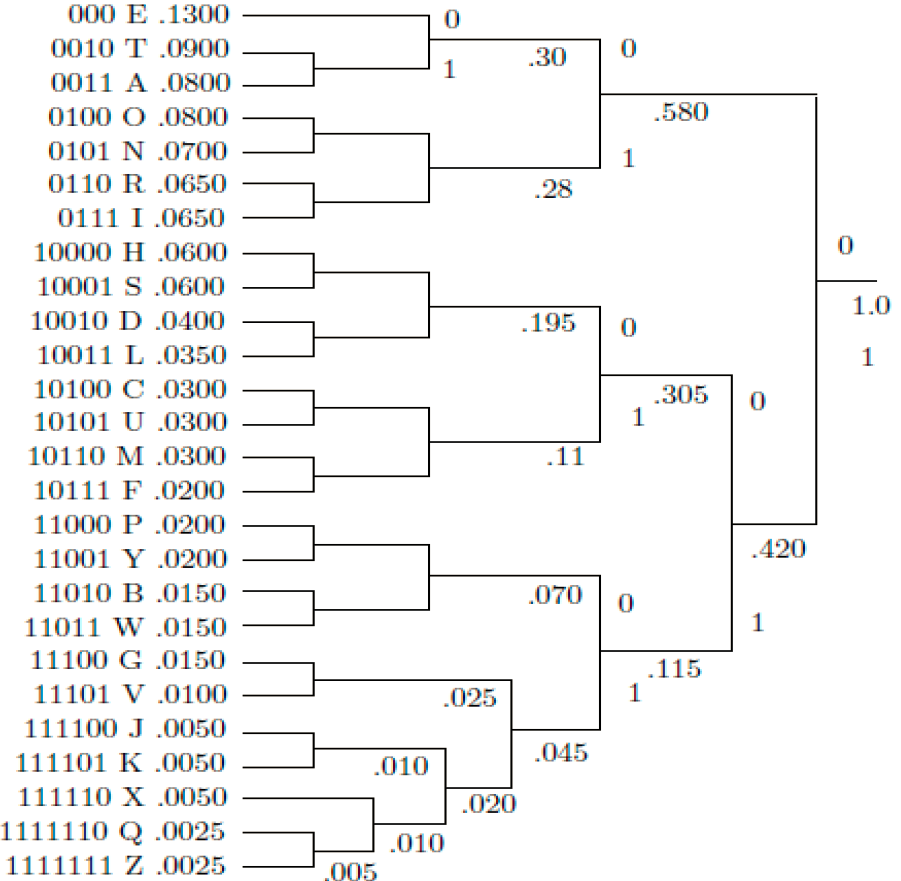
\includegraphics[width=0.8 \linewidth]{Huffman}
	\caption{Huffman coding table for English Alphabet based on character frequency}
	\label{fig:huff}
\end{figure}

P300 is widely used to provide a desired choice, a special attention or decision involuntarily and at a speed faster than the actual realization of brain. This trait of P300 makes it ideal for error detection and text input. In this application, a constant frequency flash shifting between 0 and 1 is shown as visual stimuli and the user's EEG variation would reflect their choice. The binary input could be more efficient than the original text input as the flash and decision speed could be generally faster than the mechanic input such as keyboard or touch screen.

For example, at $t = 0 ms$ a flash of 0 sign is shown to subject and at $t = 40 ms$ another flash of 1 sign is shown. The subject's desired input is 0 then at $t = 300 ms$ a positive potential fluctuation should be detected and at $t = 340 ms$ there should not be a detectable sign. Although in practice the latency caused by sensor, a generally speed of $150 ms$ per input is practical \autocite{sakai2012alphabet}. 

In a binary spelling approach, we could adopt Huffman code to compress data. Huffman code is a varied length encoding method based on Binary Search Tree. It means that the most frequently used character would have a short code, and the overall length of information could be compressed.

\subsubsection{the P300 Alphabet Matrix Layout Encoding}

\begin{figure}
	\centering
	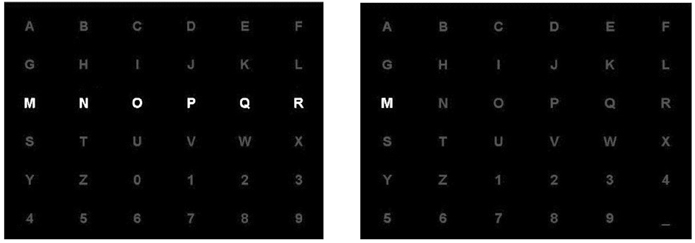
\includegraphics[width=0.8 \linewidth]{P300Spell}
	\caption{A common P300Spell interface, the layout could influence performance}
	\label{fig:P300Spell}
\end{figure}

Another popular approach would be direct alphabet based flashing matrix in front of people's eyes \autocite{sakai2012alphabet}. The decision making is two fold: first choose the row then choose the column, in this way each character is determined by a 2D coordination. One character is chosen through 2 times of choosing but the sequence need to be watched is more complicated and could bring more distraction.

\begin{figure}
	\centering
	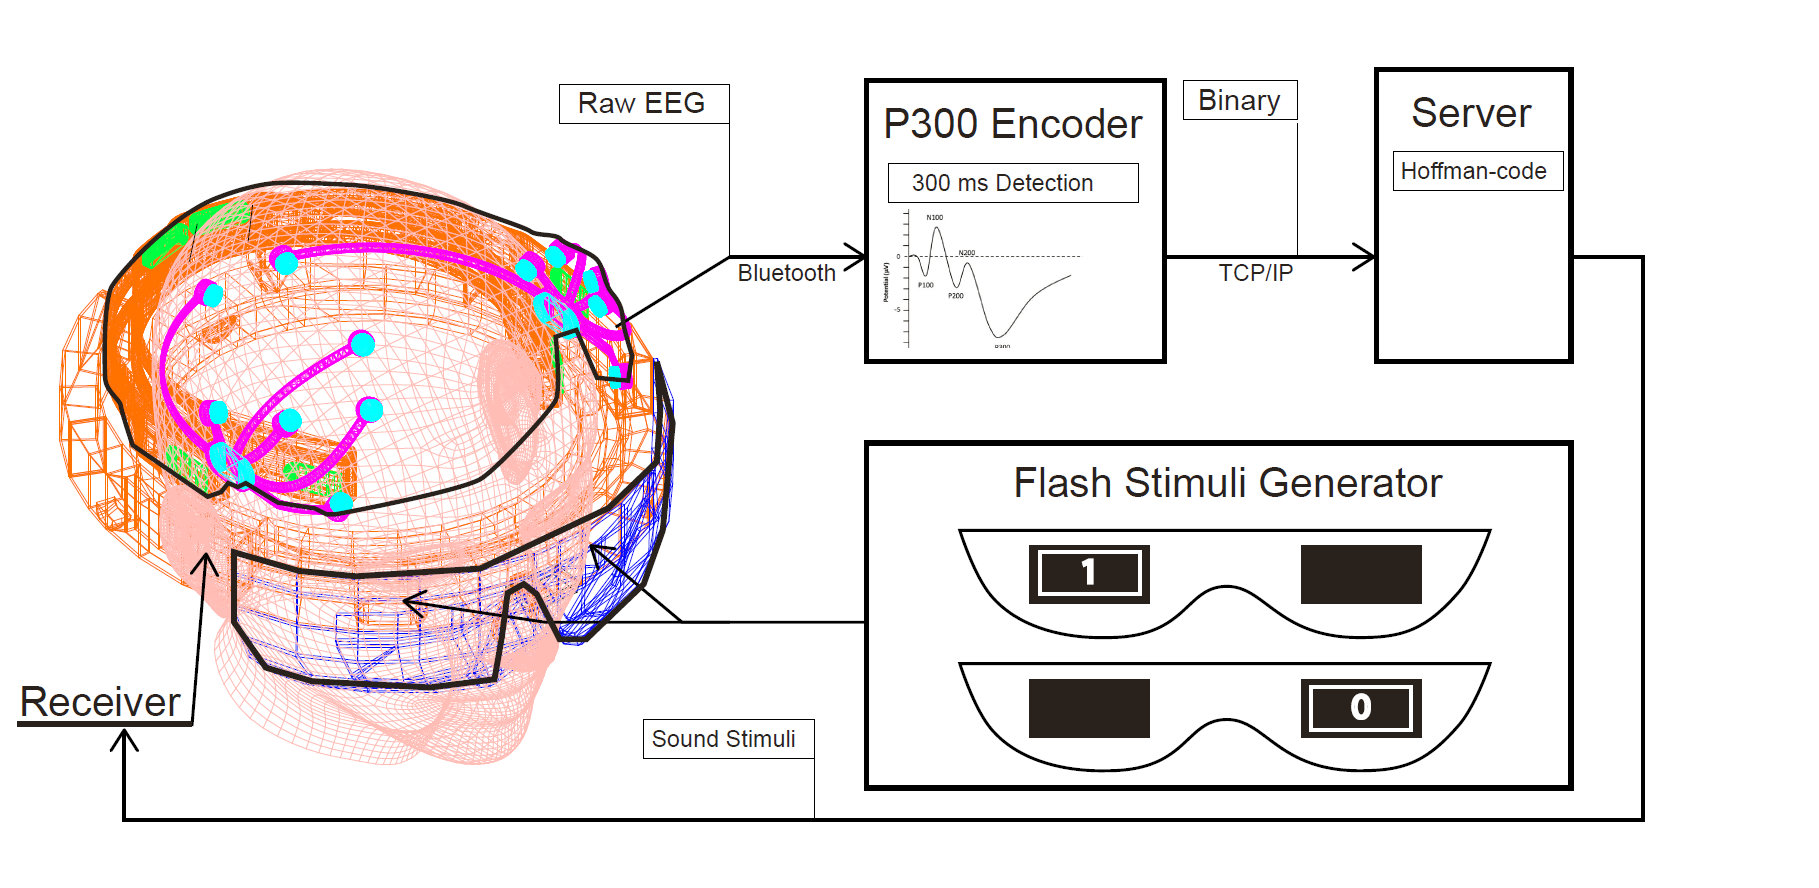
\includegraphics[width=\linewidth]{Holohead_full}
	\caption{The Composition and data flow of Binary Communication Approach}
	\label{fig:holohead}
\end{figure}

\subsection{System Implementation}

\begin{itemize}
    \item \textbf {Reader}: The hardware of mind reader is an Emotiv Epoch 16-Channel EEG headset. It captures the raw EEG data at 240HZ and sends raw EEG to \textbf{Server} by Bluetooth.
    \item \textbf {Screen}: The hardware of stimuli giver is a Microsoft Hololens. Hololens generate image overlay over the sight of people through optical technique. In a binary code approach, the choice sequence is presented on left eye and right eye respectively. In a matrix approach, the choice sequence is presented only on one of the eye screen. The user could concentrate on other tasks while doing this type of text inputting.
    \item \textbf {Server}: The server is a Thinkpad X1 Carbon with Win 10 Pro running the software. The server filters and de-noises the raw EEG data send from Emotiv \textbf{Reader}, and then detect the P300 signal to reverse calculate the input of user. \\
    According the encoding method user has set, the choice of user is either decoded as hoffman code or as spell matrix and finally converted to ASCII code. The user can chose the destination of sending this piece of information and the information would be send through TCP protocol after TTS.   
    \item \textbf{Receiver}: The actuator is integrated with Microsoft Hololens and upon receiving the sound signal and play to the target user.
\end{itemize}

\subsection{Conclusion and Discussion of Encoded Communication Approach based on ERP}

This prototype is a novel implementation of classical P300 spelling machine using augmented reality. Compared with the classical approach, it has advantage such as portable, possible to conduct multi-user chatting, and fine for multi-tasking. 

Instead of the computer screen, the visual stimuli of this prototype is projected on Microsoft Hololens and appears like a hologram, which allow user to pay visual attention on the environment without being stuck on the text input task. Besides the speller, the device also contains a receiver which could be used to receive message sent from other user on the server.

The potential problem is, although researchers have proved that visual design does matter\autocite{sakai2012alphabet}, the precise threshold of visual flash to generate P300 is currently unclear. Whether the luminosity of Hololens is strong to produce P300 and how much it would be effected is unknown.

Another obvious noise source is also brought by Hololens. Since the device allows multitasking, it would involve the other choice and decision making when text input. Some of the noise could be filtered considering the frequency of stimuli is constant, but it could be hard to fully separate the noise from irrelevant decision making purely by timing and EEG signal. A better input interface with confirmation could be a manual fix to this problem but imperfect.  

\section{Emotional Sharing Approach based on ERD/ERS}

The prototype read the emotion state of user based on an implicitly and involuntarily criteria. It circumvent any kind of output organ, either facial expression, voice or body movement in terms of emotion expression. Then it is capable of sharing the current emotion state to anywhere with internet connection.

Aimed to help people express feeling, The prototype reads and share users' feeling . The users could not choose not to send her mind state nor not receiving others. It could be interpreted as a device from one of future dystopia where everyone has no secret feelings.

\subsection{Design Consideration}

This application reads the raw EEG of the subject at first. Then through Bluetooth communication, it send the raw electrode potential to the server. The server would do pre-processing of data such as filtering and Fast Fourier Transformation to extra the ERD/ERS parameter of subject.

Then the server would put it into a pre-trained Random Forest model. The detailed training procedure such as database chosen would be introduced in later section. The random forest model could be viewed a collection of decision tree. Using a majority voting technique, the random forest model, like decision tree, is easy to train and use for pattern finding task and widely used in natural language processing even now. The pre-trained model would take the 14-channel band power (ERD/ERS) as input and reproduces a 3-dimensional emotion coordinate on: Arousal, Valence and Dominance. This 3-dimensional is named PAD model, it is a classical emotion description model widely adopted.\autocite{bakker2014pleasure}

Then the emotion coordinate is converted into 8 categories of emotions: \{Excitement, Range, Anguish, Surprise, Enjoyment, Terror, Humiliation, Disgust\}. The categories are turned into voical signal through TTS, and transmitted through TCP server to the Receiver of another user. So, the receiver would tell the emotion that one user has to another.

\subsection{System Implementation}

The prototype is composed of 3 parts:

\begin{itemize}
    \item \textbf {Reader}: The hardware of mind reader is an Emotiv Epoch 16-Channel EEG headset. It captures the raw EEG data at 240HZ and sends raw EEG to \textbf{Server} by Bluetooth.
    \item \textbf {Server}: The server is a Thinkpad X1 Carbon with Win 10 Pro running the software. The software would first filter the data, remove artifacts such as eye movement or acceleration \autocite{le2011method} \ref{fig:FFT}. Then the cleaned data would go through Fast Fourier Transformation mapping into band power. The band power would be send to a pre-trained \textbf{Model}: A Random Forest based emotion classifier. For each class, a score would be scaled to 0-9. A regression is conducted first and then converted into binary value on 3 dimensional, which contains [high/low arousal, high/low valence, high/low dominance]. The three bool information would be then converted to one of the eight emotions [Excitement: HHH, Joy: LHH, Contempt: LHL, Surprise: HHL, Anger: HLH, Distress: HLL, Fear: LLH, Shame: LLL] would be passed through Speech Synthesis and send to the \textbf{Receiver}.
    \item \textbf{Receiver}: The actuator is as simple as a wireless earpod receiving the synthesized sound from \textbf {Server} and play the sound to people wearing it.
\end{itemize}

When put on and connected to the Server, the device would iterative send EEG data to the server. The server would estimate the distance between users by Bluetooth signal strength. When two users are close enough, the server would send the synthesized sound containing her emotion state description to each other iterative.

In this way, the emotion condition could be shared between people involuntarily.

\begin{figure}
	\centering
	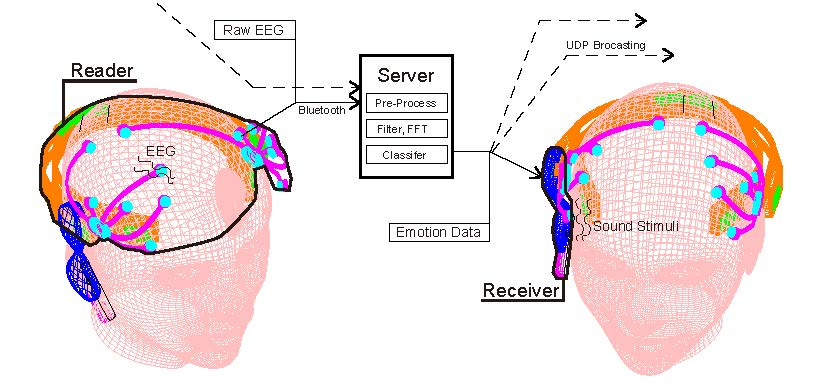
\includegraphics[width=\linewidth]{Diagram_2}
	\caption{The Composition and data flow of Emotional Sharing Approach}
	\label{fig:Lietome}
\end{figure}

\subsection{Data Pre-processing}

\begin{figure}
	\centering
	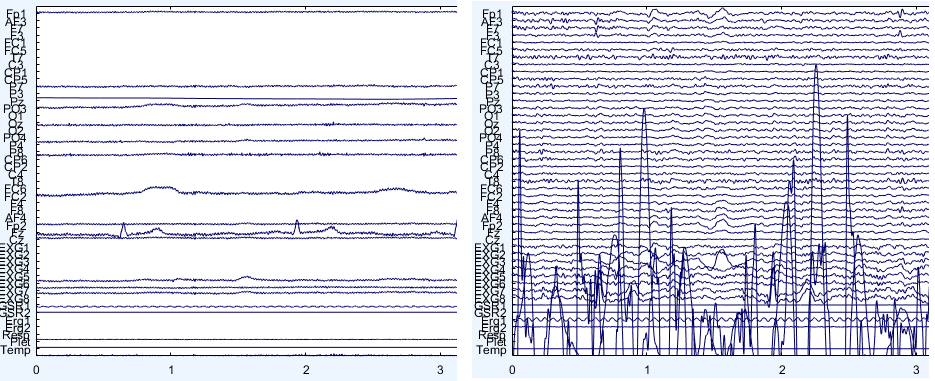
\includegraphics[width=0.8\linewidth]{Deap_Preprocess}
	\caption{A sample of unfiltered (left) and filtered (right) data}
	\label{fig:filter}
\end{figure}

The DEAP dataset\autocite{koelstra2012deap} is preprocessed in Matlab with EEGLab with following procedure: down-sampled from 512Hz to 128Hz, EOG artifacts remove by ICA, a bandpass filter [4.0-45.0] Hz applies, and reorders with Subject ID from 1-32. Each subject is asked to perform 40-trails, each trail is composed of a 2 sec informative screen, a 5 sec baseline, a 1 minute display of video and a self-assessment score sheet. The sheet from subjects are regarded as ground truth, this include a a discrete 9-point scale for valence, arousal, dominance and like and a 5-point scale for familiarity for each video. 

\begin{figure}
	\centering
	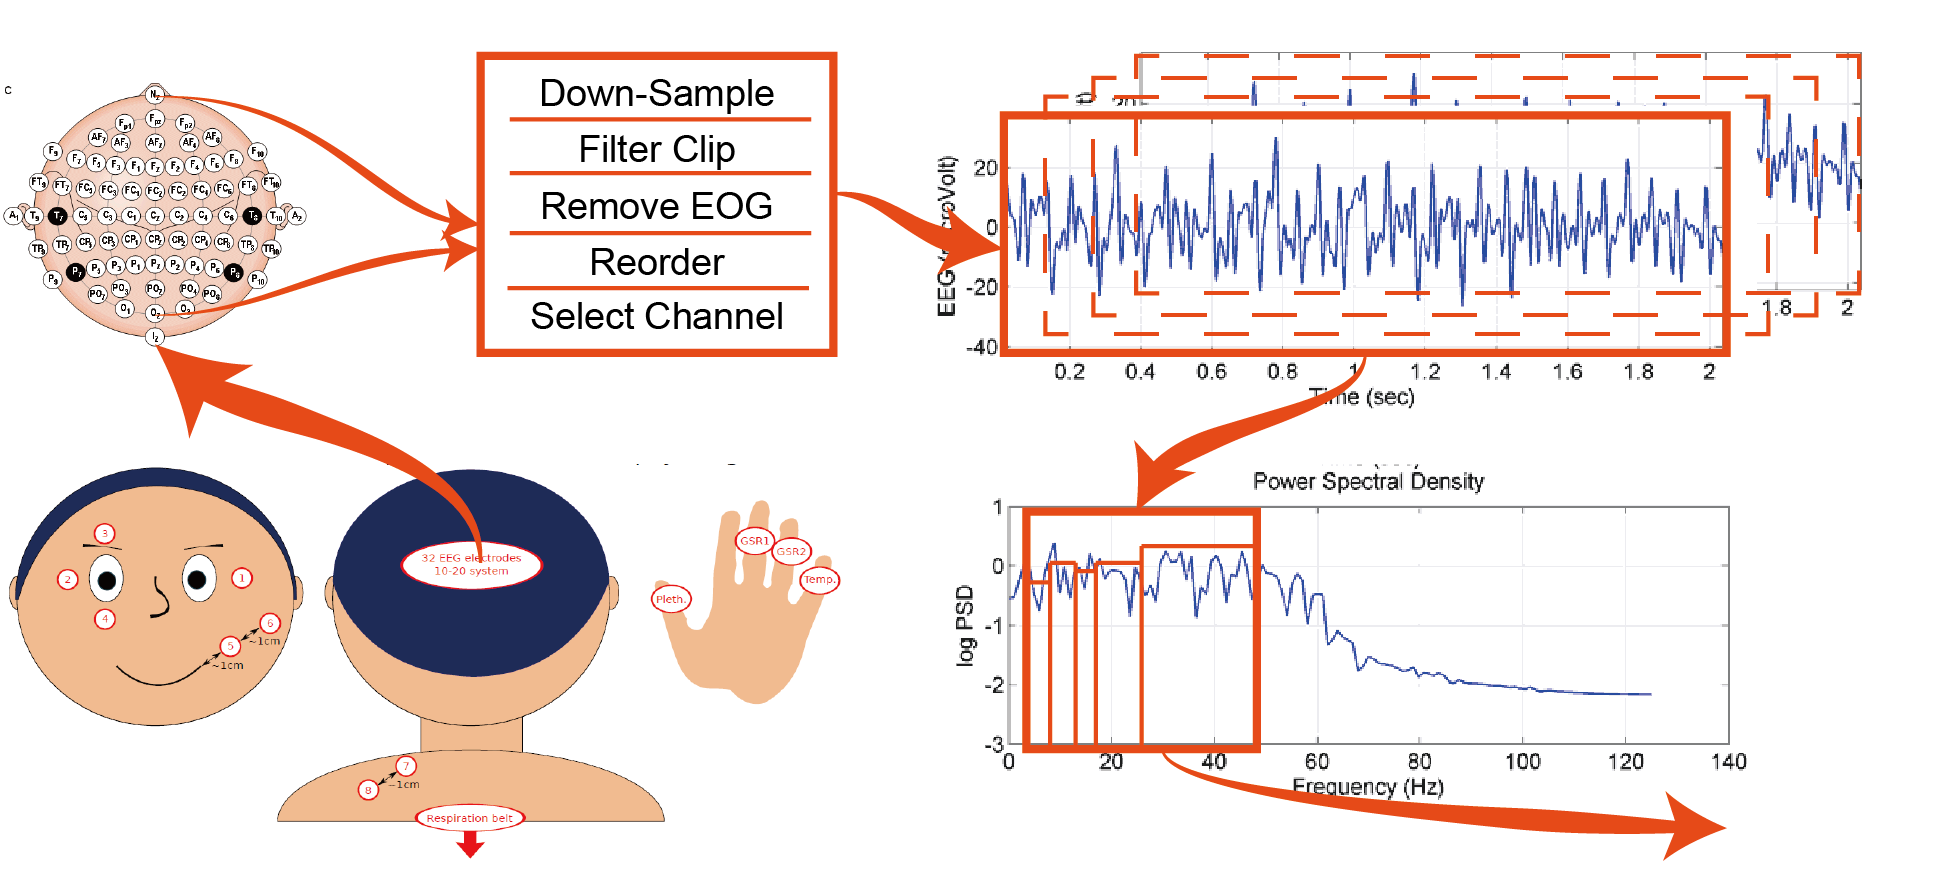
\includegraphics[width=\linewidth]{Diagram_FFT}
	\caption{The pre-processing procedure diagram}
	\label{fig:FFT}
\end{figure}

After data filtering and matching, a Fast Fourier Transformation(FFT) is performed in Python with PyEEG to calculate band powers. The band powers are selected as follows: [4-8]Hz theta band, [8-12]Hz alpha band, [12-16]Hz low beta band, [16-25]Hz high beta band and [25-45]Hz gamma band. To satisfy the standard of Emotiv, the channel chosen from 10-20 system is [AF3, F3, F7, FC5, T7, P7, O1, AF4, F4, F8, FC6, T8, P8, O2].

\subsection{Model Selection and Training}

Some researchers convert directly from the 0-9 score to 0/1 binary category and then conduct classification. This is an intuitive approach however lose the ranking information of each user toward each video. In this paper, the raw score is adopted directly and feed into regression model instead of classification model, and later the regression result is converted into binary category. 

\begin{table}[]
\begin{tabular}{llllll}
\hline
& SVM & RF & Ada & ANN 500 & ANN 3000 \\ \hline
Accuracy H/L Valence & 60.5\%                 & \textbf{83.7\%}         & 61.5\%   & 59.1\%         & 81.4\%          \\
Regression Error          & 1.62                   & \textbf{1.09}          & 1.92     & 1.76           & 1.35 \\ \hline           
\end{tabular}
\caption{Cross Model Comparison: SVM: Support Vector Machine, RF: Random Forest, Ada: AdaBoost, ANN 500: Artificial Neural Network epoch = 500}
\end{table}

Several popular regression algorithm are selected such as Support Vector Regressor, Random Forest Regeressor, AdaBoost Regressor and Artificial Neural Network. As tested, the Random Forest generally out perform other model with minimal training time and light weight. An random forest with Minimum Number of Sample Leaf = 2 and Number of Estimator = 512 is chosen for best performance, and the model performs fair on all three categories. For binary classification, [Arousal = 82.7 \%, Valence = 83.7\%, Dominance = 81.8\%, Liking = 85.1\%].

\begin{table}[]
\begin{tabular}{llllll}
\hline
            & N Es 10   & N Es 100  & N Es 250  & N Es 512  & N Es 750  \\ \hline
Min Leaf 2  & 77.4\% & 81.5\% & 83.0\% & \textbf{83.7 \%} & 82.1\% \\ 
Min Leaf 10 & -      & 76.2\% & -      & -      & -      \\
Min Leaf 50 & -      & 68.2\% & -      & -      & -     \\\hline
\end{tabular}
\caption{Random Forest Regression Parameter Tuning: N Es: Number of Estimator, Min Leaf: Minimum Number of Sample Leaf}
\end{table}

\subsection{Conclusion and Discussion of Emotional Sharing Approach based on ERD/ERS}

This prototype presents a ERD/ERS based telepathy approach through brain-computer interface. It read the emotion state of one user and share it with others where-ever internet access is possible. The general process is implicit and not-open to user control. One sub-routine of this project also improve the standard process of emotion classification. It uses the score of subject not only as a binary category indicator but also as a rank technique. In this way it improve the general accuracy using machine learning method over DEAP database.

A major problem of prototype implement is that only one Emotiv EEG headset could be afforded, since the amount of fund received by this project is limited to 500\$. The prototype losses lots of convincing without a multi-user demo presented. Another problem the over-expression issue. Research also reveal that over-expression of emotion could cause problem \autocite{bonanno2004importance}. Despite the prototype could distinguish negative emotion with positive emotion, it could not judge the context to express them properly.

On the model training side, the model is trained on a subject dependent. Which means the accuracy of model is based on the fact that training data-set and testing data-set contains same subject. While subject independent modeling should be adopted since this would produce a universal result where different subject could use the same model, despite the fact that ERD/ERS based emotion classification is quite limited to per-subject based experiment. The pattern of subject's emotion and EEG is quite individual based according to current research method.

\section{Conclusion and Discussion}

This paper discuss the concept of telepathy and, historical and modern implement of telepathy and describe two telepathy prototype based on brain-computer interface. The first implement integrate mixed reality with P300 signal spelling. This enhances the portability and usability of BCI based spelling machine. The other use a pre-trained model based on DEAP data-base. It improves the accuracy of DEAD based emotion using rank extraction technique. It also provides a demo forcing the emotion sharing among people. 

Both of the prototype is envision based and not fully functional due to lack of funds and equipment. It would be better for me to build them up for my thesis or other studio next years.

\section{Acknowledgement}

Thanks Dr. Matthew Hockenberry for teaching me media theory during the whole semester. The lectures and read lists are incredibly helpful. Thanks Mrs. Rebecca G Silver from NYU Wassermann Center for providing fund to the equipment, so I could afford the Emotive EEG headset. Thanks to my friends Sara and Mingming for giving me advice on English grammar.

\printbibliography

\end{document}